% !TEX encoding = UTF-8 Unicode

\chapter{Sample Results}
\label{chap:results}

%%%%%%%%%%%%%%%%%%%%%%%%%%

\section{When New York meets Van Gogh}

The first sample output here is overlay Van Gogh's starry night\footnote{Vincent Van Gogh,
Starry Night (1889)}
on a picture of New York\footnote{The author took this photo in May 2017}.

    \begin{figure}[!hbt]
    \center
    \subfigure[New York photo]{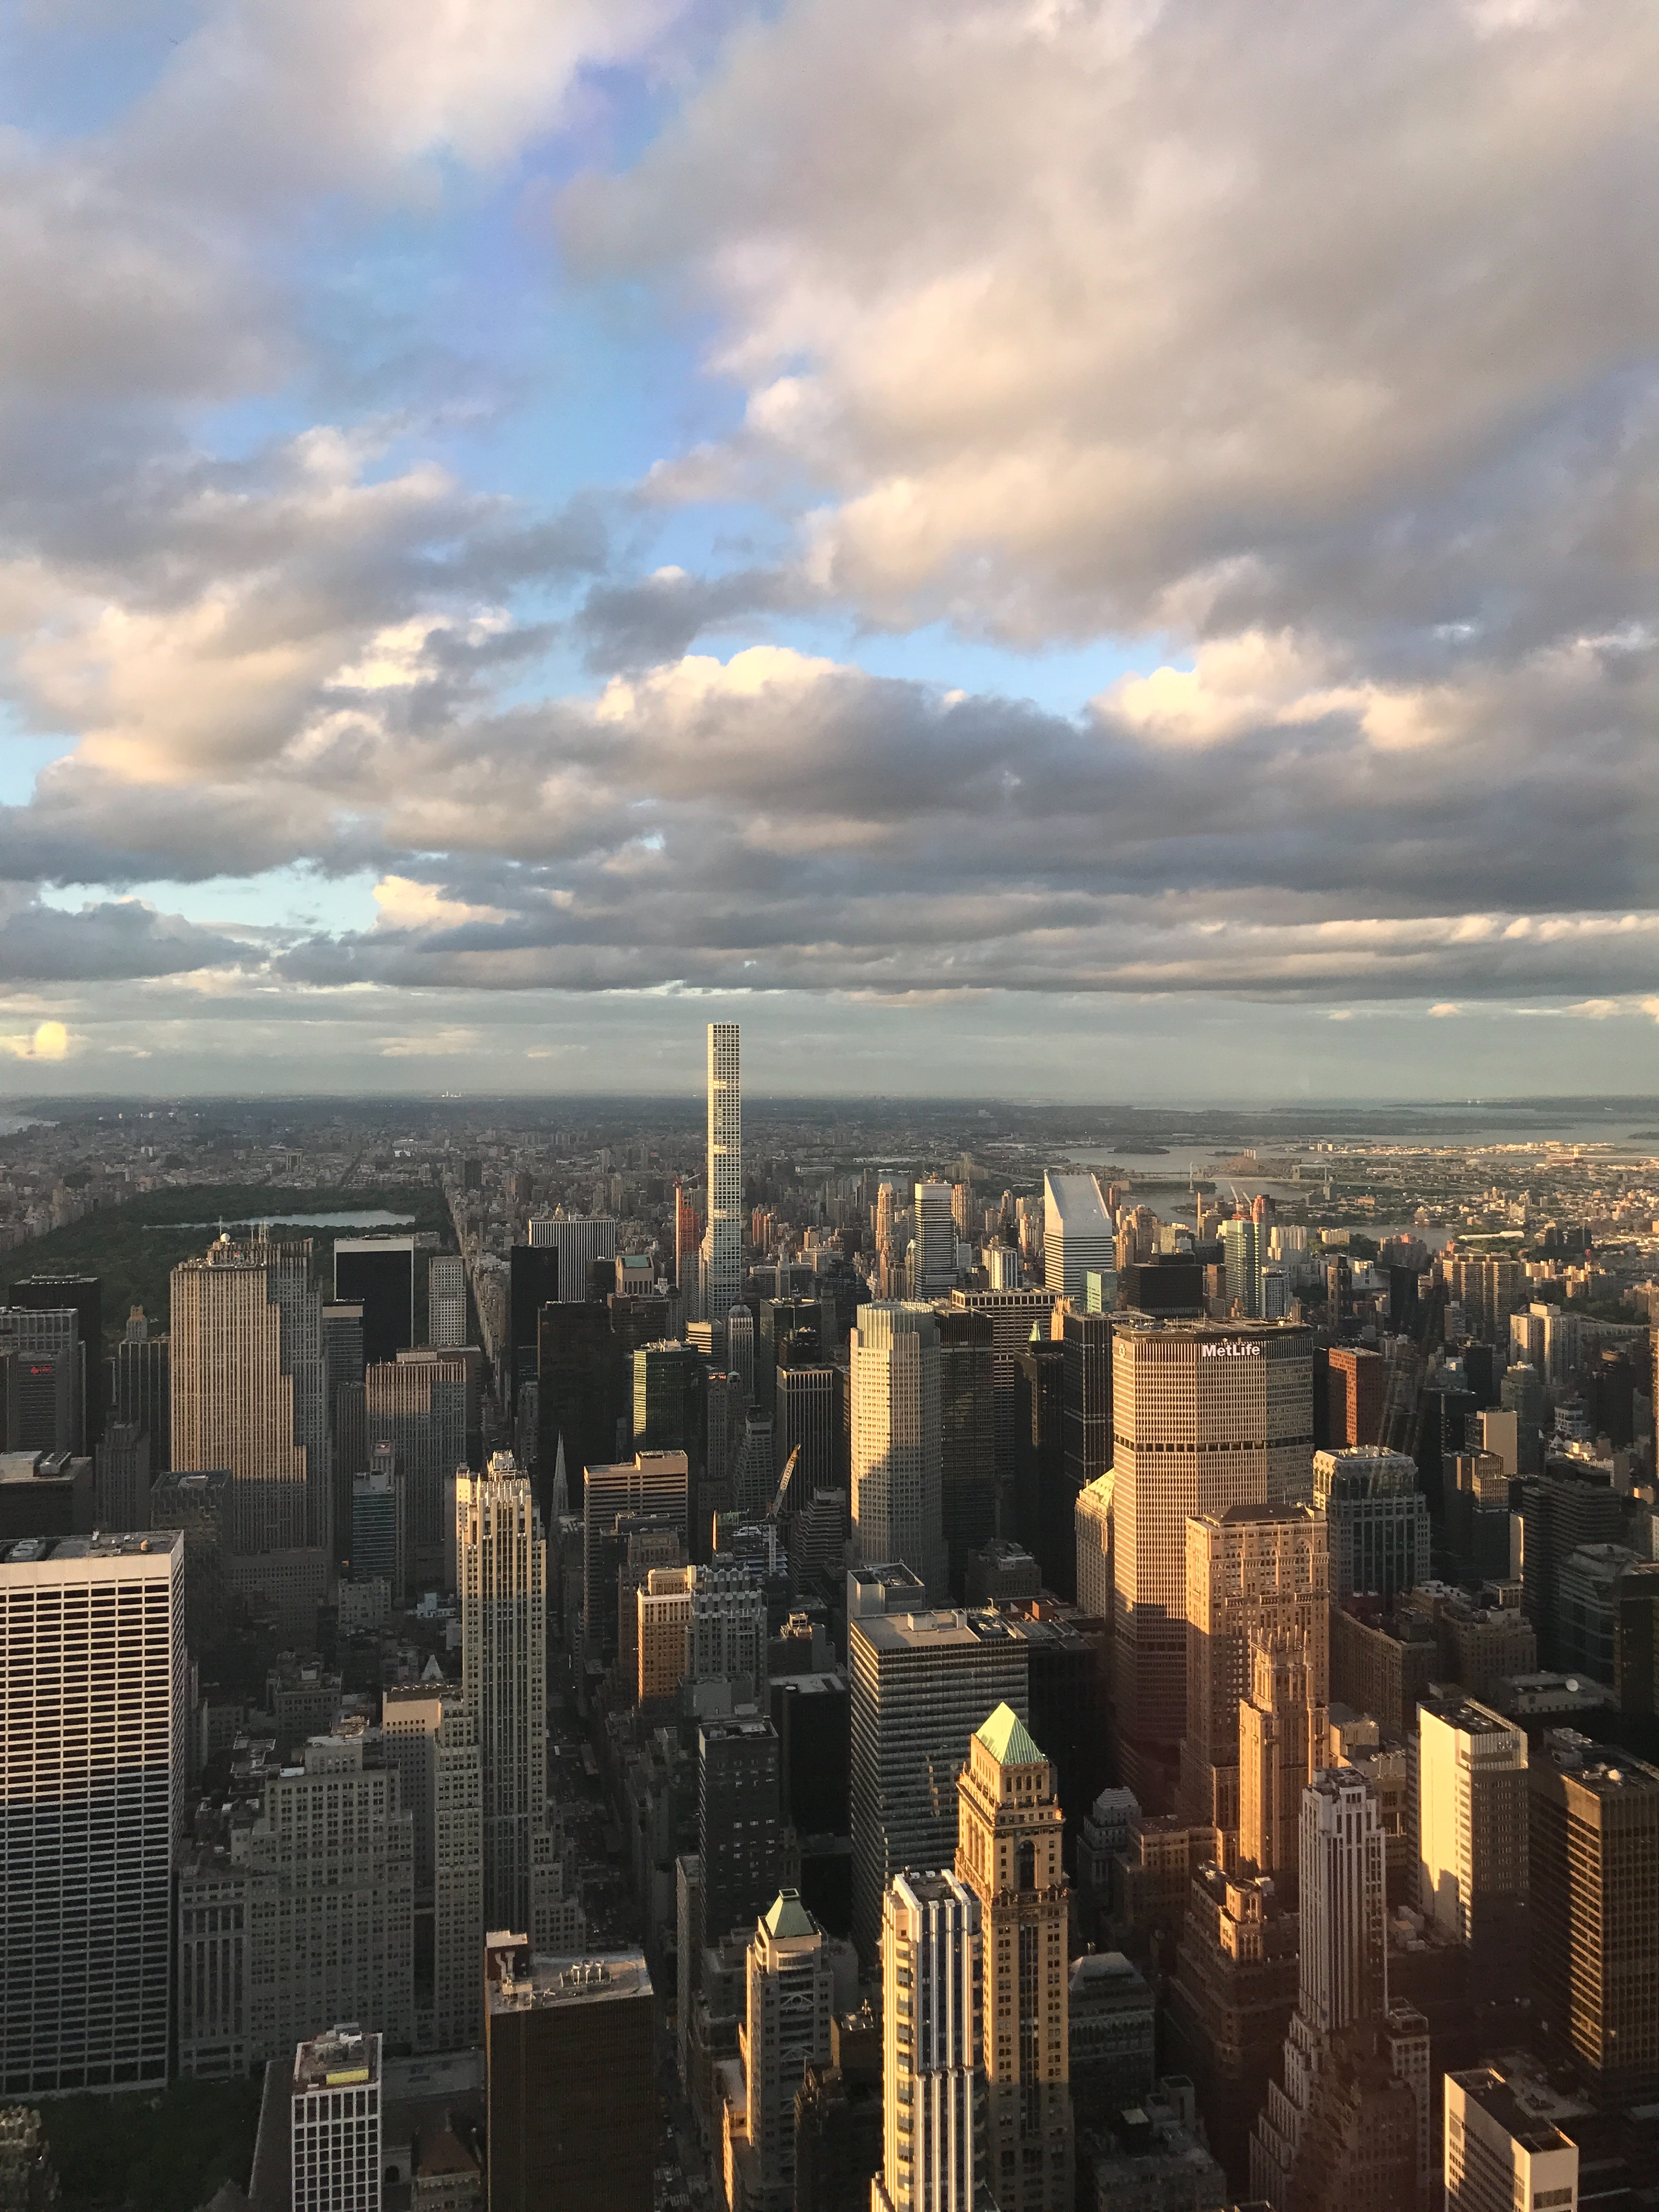
\includegraphics[height=12em]{input/new_york.jpg}}
    \subfigure[Van Gogh Starry Night]{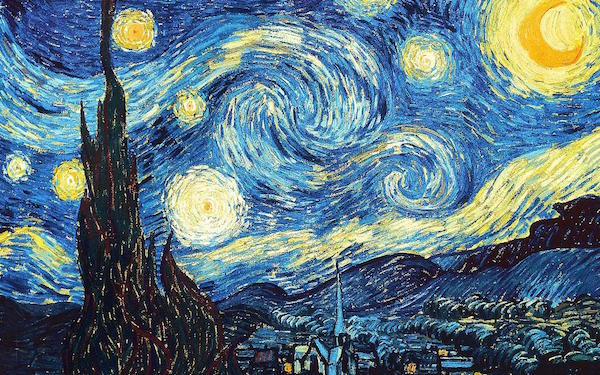
\includegraphics[height=8em]{input/van_gogh.jpg}}
    \caption{Raw input of New York photo and Van Gogh painting}
    \label{fig:results:vg:origin}
    \end{figure}

With default parameters specified in Sec.\,\ref{sec:implementation:parameters},
we have the output graph below as Fig.\,\ref{fig:results:vg:final}

    \begin{figure}[!hbt]
    \center
    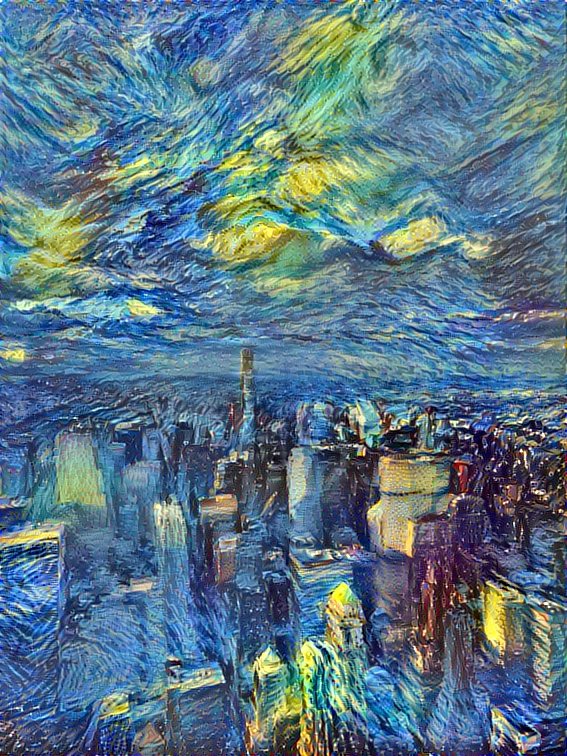
\includegraphics[width=0.3\textwidth]{output/vg_final.jpg}
    \caption{Overlay Starry Night on New York}
    \label{fig:results:vg:final}
    \end{figure}


\subsection{Checkpoint output}
\label{sec:results:vg:checkpoint}

By default, we set number of iteration to 1000, and save intermediate results every 100 steps.
In Fig.\,~\ref{fig:results:vg:checkpoint}, we list the output image at each checkpoint $N$,
including the initial white noise graph.

    \begin{figure}[!hbt]
    \center
    \subfigure[$N = 0$, white noise]{
\includegraphics[width=0.2\textwidth]{output/vg_0.jpg}}
    \subfigure[$N = 100$]{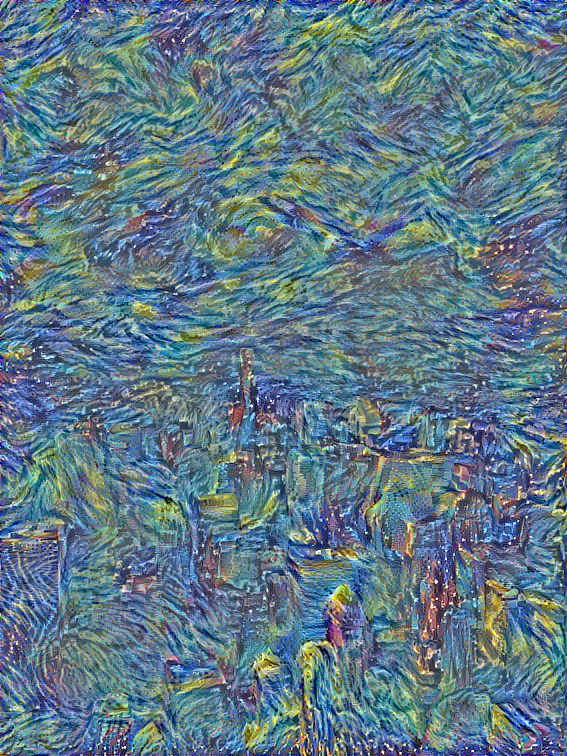
\includegraphics[width=0.2\textwidth]{output/vg_100.jpg}}
    \subfigure[$N = 200$]{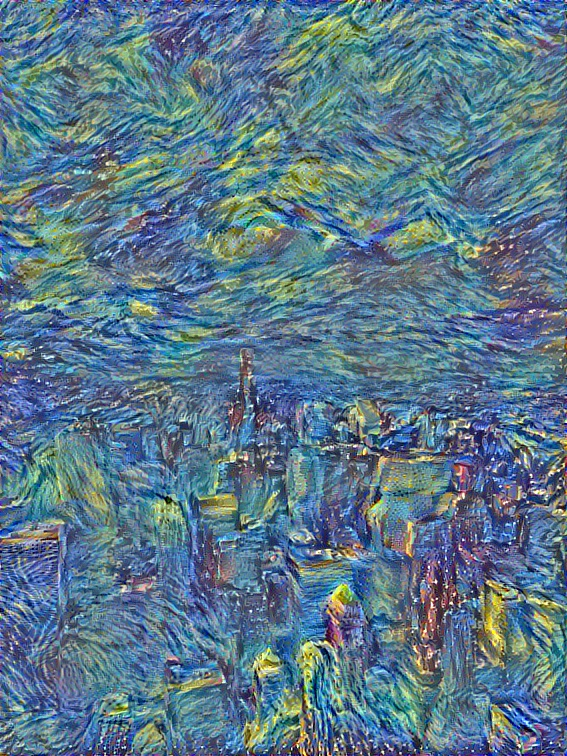
\includegraphics[width=0.2\textwidth]{output/vg_200.jpg}}
    \subfigure[$N = 300$]{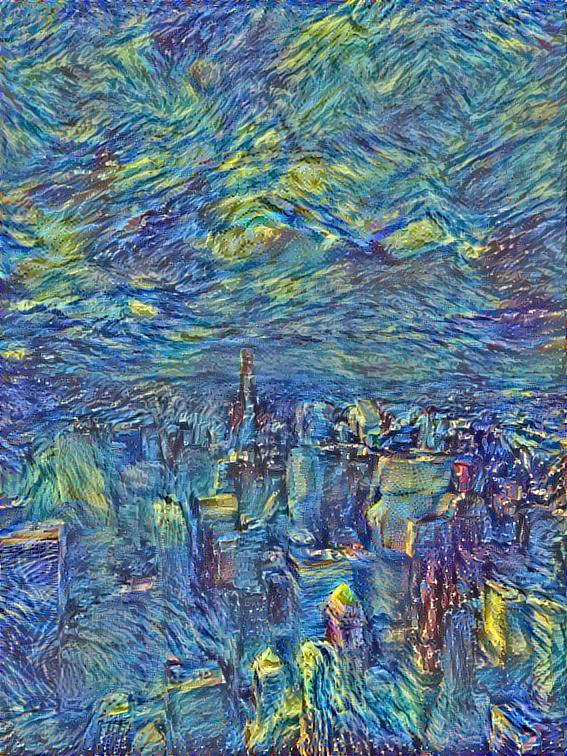
\includegraphics[width=0.2\textwidth]{output/vg_300.jpg}}
    \subfigure[$N = 400$]{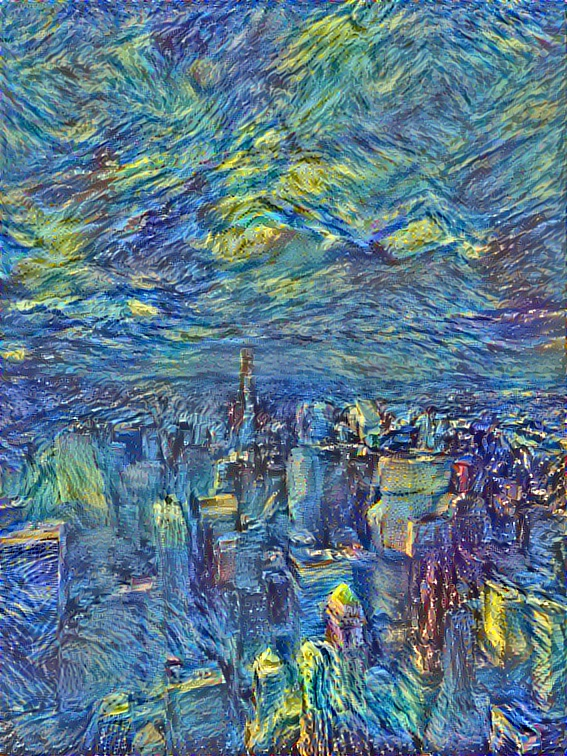
\includegraphics[width=0.2\textwidth]{output/vg_400.jpg}}
    \subfigure[$N = 500$]{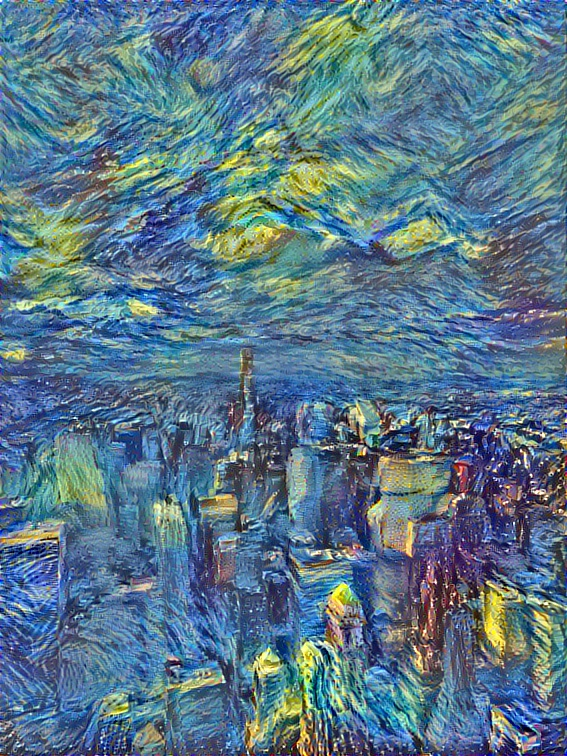
\includegraphics[width=0.2\textwidth]{output/vg_500.jpg}}
    \subfigure[$N = 600$]{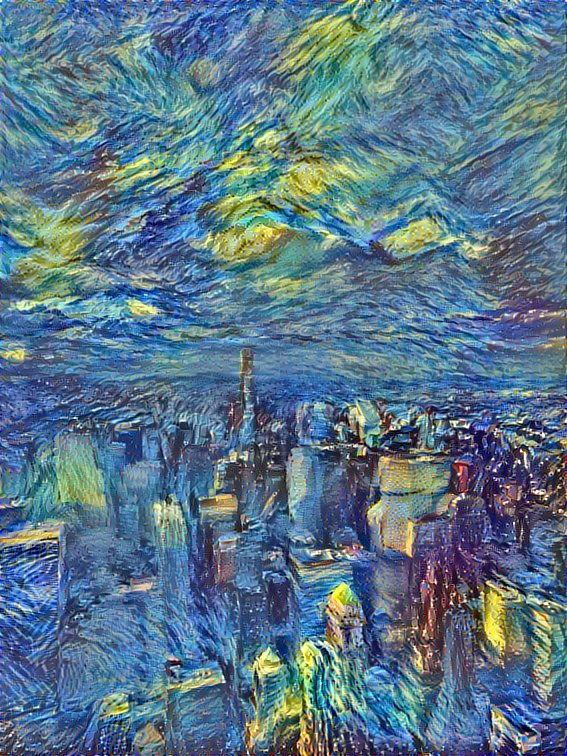
\includegraphics[width=0.2\textwidth]{output/vg_600.jpg}}
    \subfigure[$N = 700$]{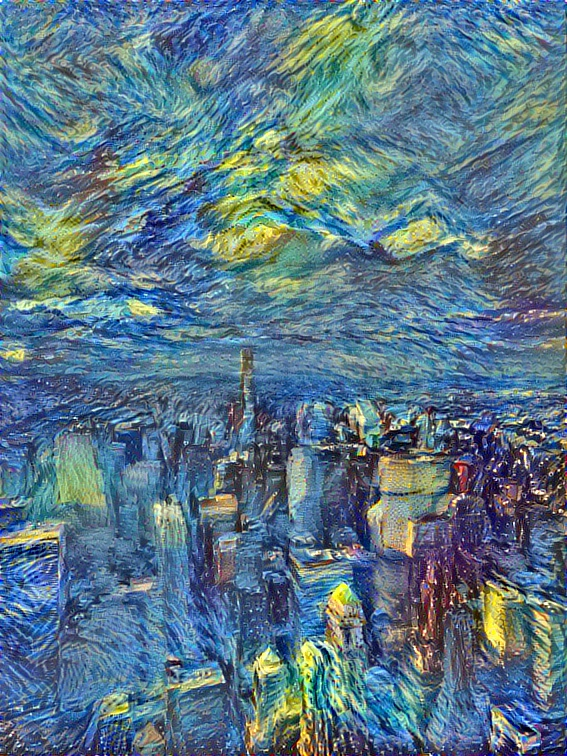
\includegraphics[width=0.2\textwidth]{output/vg_700.jpg}}
    \subfigure[$N = 800$]{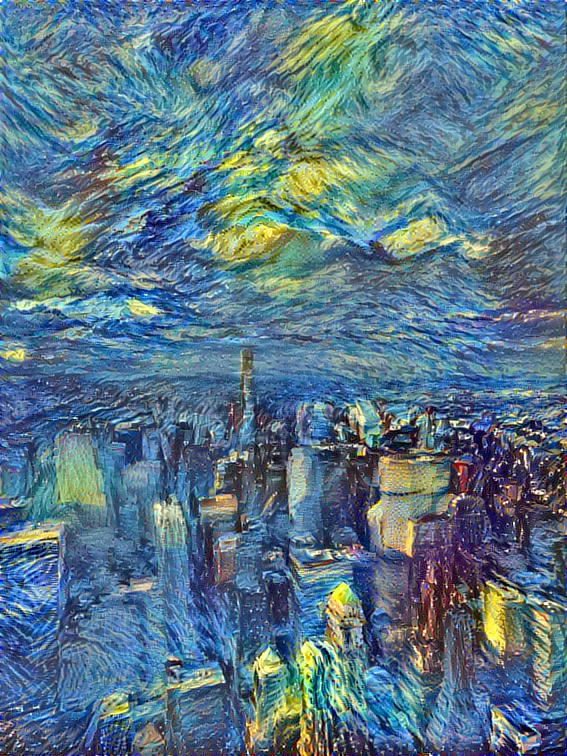
\includegraphics[width=0.2\textwidth]{output/vg_800.jpg}}
    \subfigure[$N = 900$]{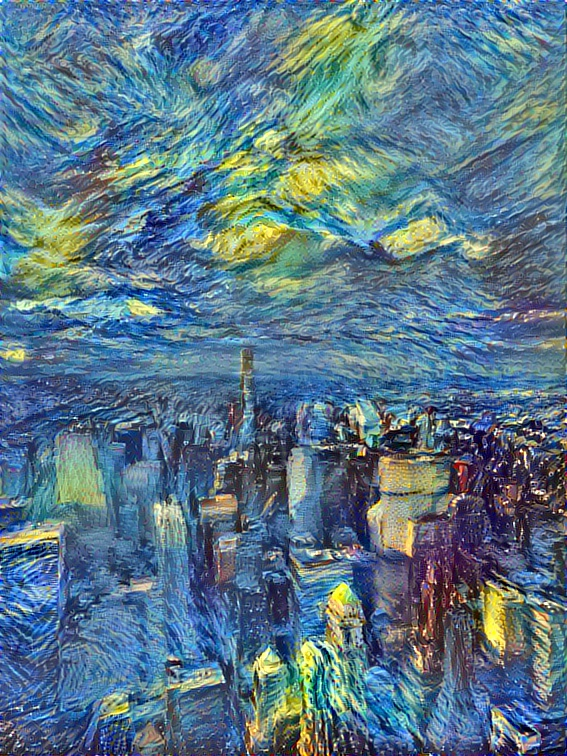
\includegraphics[width=0.2\textwidth]{output/vg_900.jpg}}
    \subfigure[$N = 1000$, final]{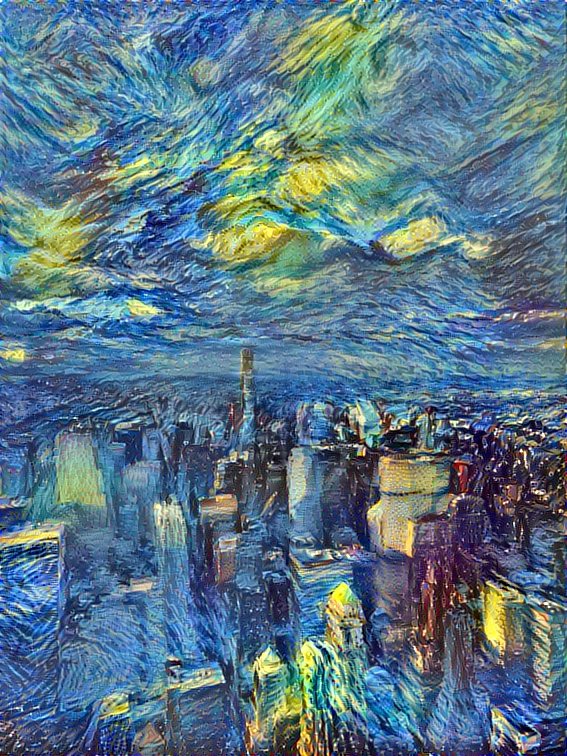
\includegraphics[width=0.2\textwidth]{output/vg_final.jpg}}
    \caption{Raw input of New York photo and Van Gogh painting}
    \label{fig:results:vg:checkpoint}
    \end{figure}

As is shown from the illustration above, the initial learning rate of the algorithm is fast
and then the speed slows down; the output result has almost converged after $N=500$.
This pattern fits the common process of other deep learning algorithms.

\subsection{Loss convergence}
As is pointed out in Sec.\,\ref{sec:results:vg:checkpoint},
total loss declines rapidly at initial stage and then converges around $N = 600$.
Fig.\,~\ref{fig:results:vg:loss} shows the loss function values at each iteration.
The concave shape of total loss can be viewed as a proof of the finding.



%%%%%%%%%%%%%%%%%%%%%%%%%%

\section{More examples}

We also performed a few more experiments with other artistic styles.
Among many artists who have a very strong characteristic and aesthetic style,
we chose Pablo Picasso and Jackson Pollock as two examples.
Furthermore, the works we chose
(Guernica by Picasso\footnote{Pablo Picasso, Guernica (1937)} and
Number 30 by Pollock\footnote{Jackson Pollock, Autumn Rhythm (Number 30, 1950)})
both have a very strong and identifiable style.

In Fig.\,~\ref{fig:results:pp} and Fig.\,~\ref{fig:results:jp} we present
the original photo, artistic work, and style tranferred output picture.

    \begin{figure}[!hbt]
    \center
    \subfigure[New York photo]{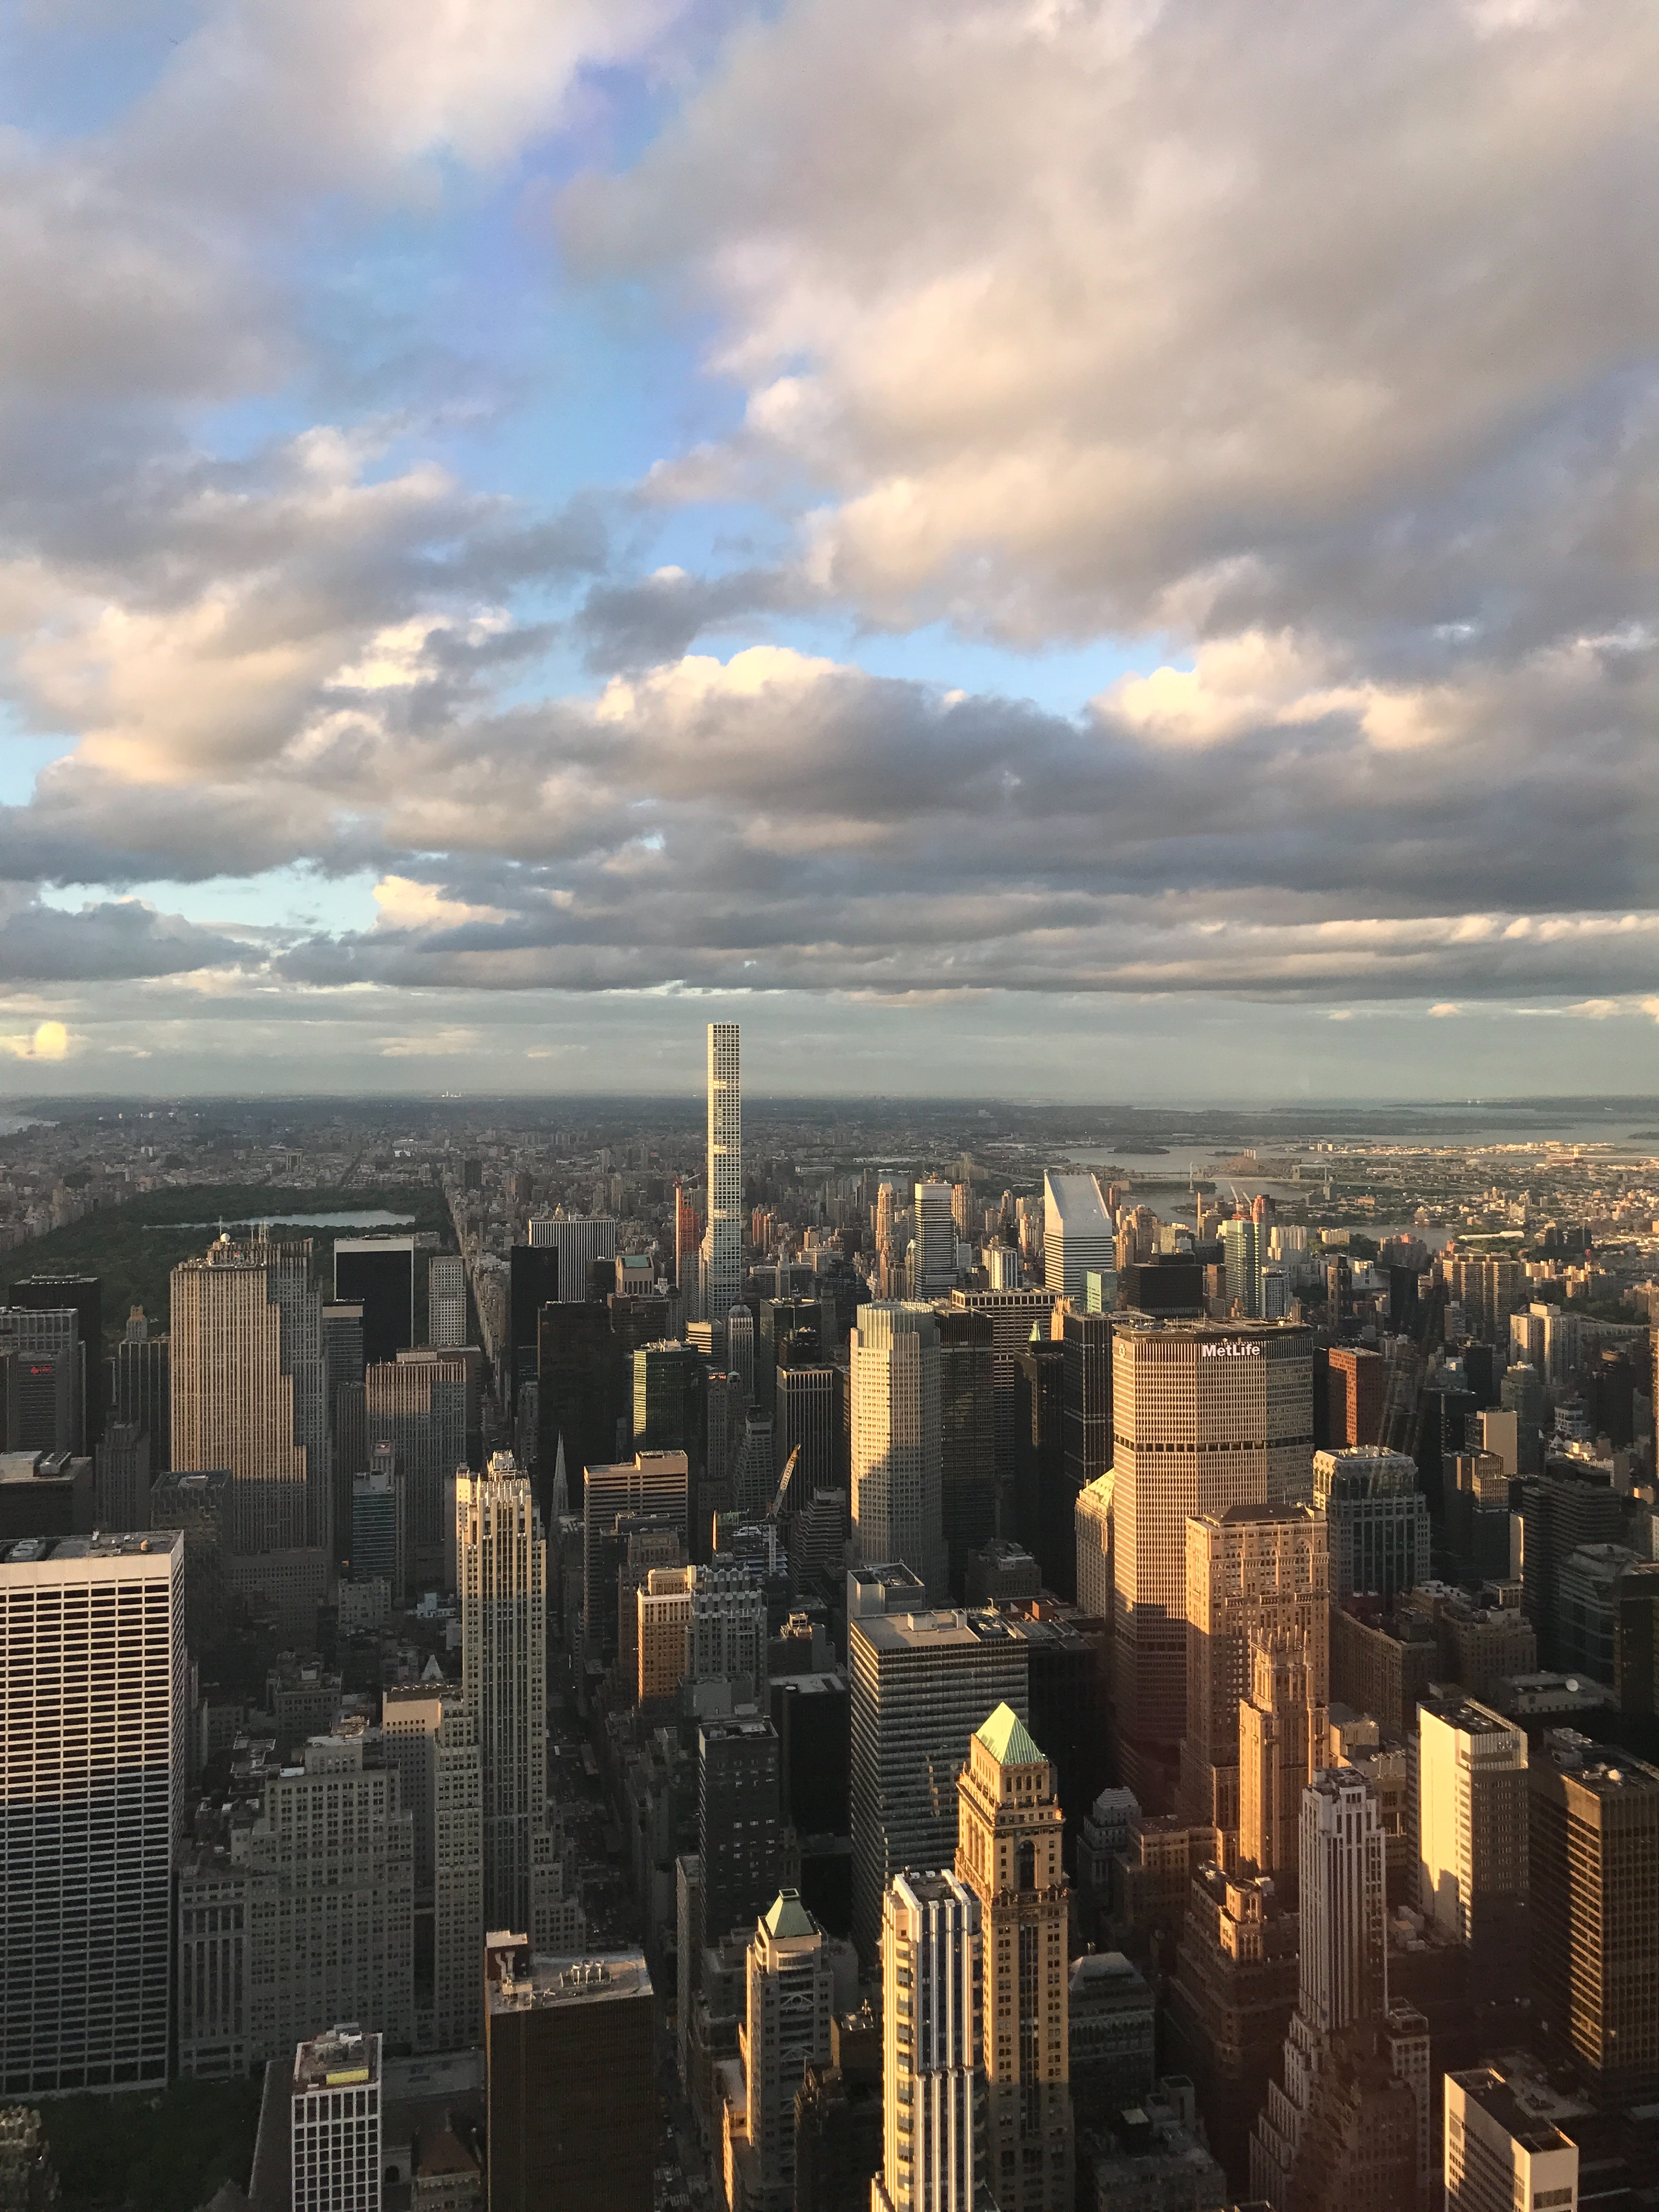
\includegraphics[height=12em]{input/new_york.jpg}}
    \subfigure[Pablo Picasso Guernica]{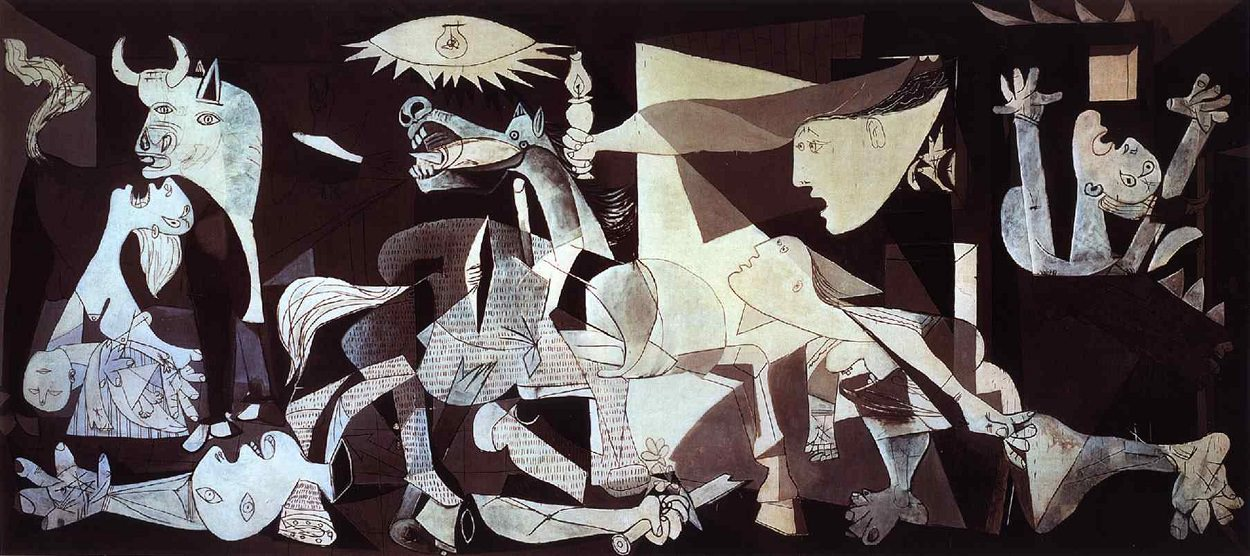
\includegraphics[height=8em]{input/pablo_picasso.jpg}}
    \subfigure[Style tranferred output]{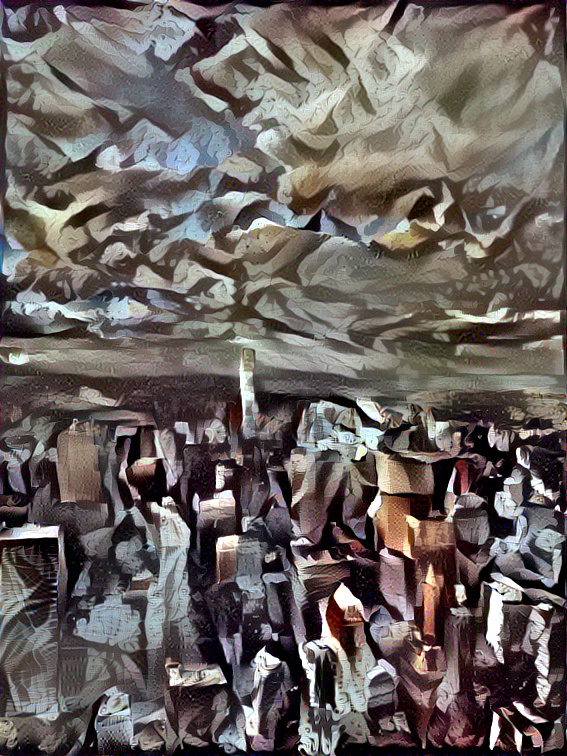
\includegraphics[height=12em]{output/pp_final.jpg}}
    \caption{Overlay Picasso on New York}
    \label{fig:results:pp}
    \end{figure}

    \begin{figure}[!hbt]
    \center
    \subfigure[New York photo]{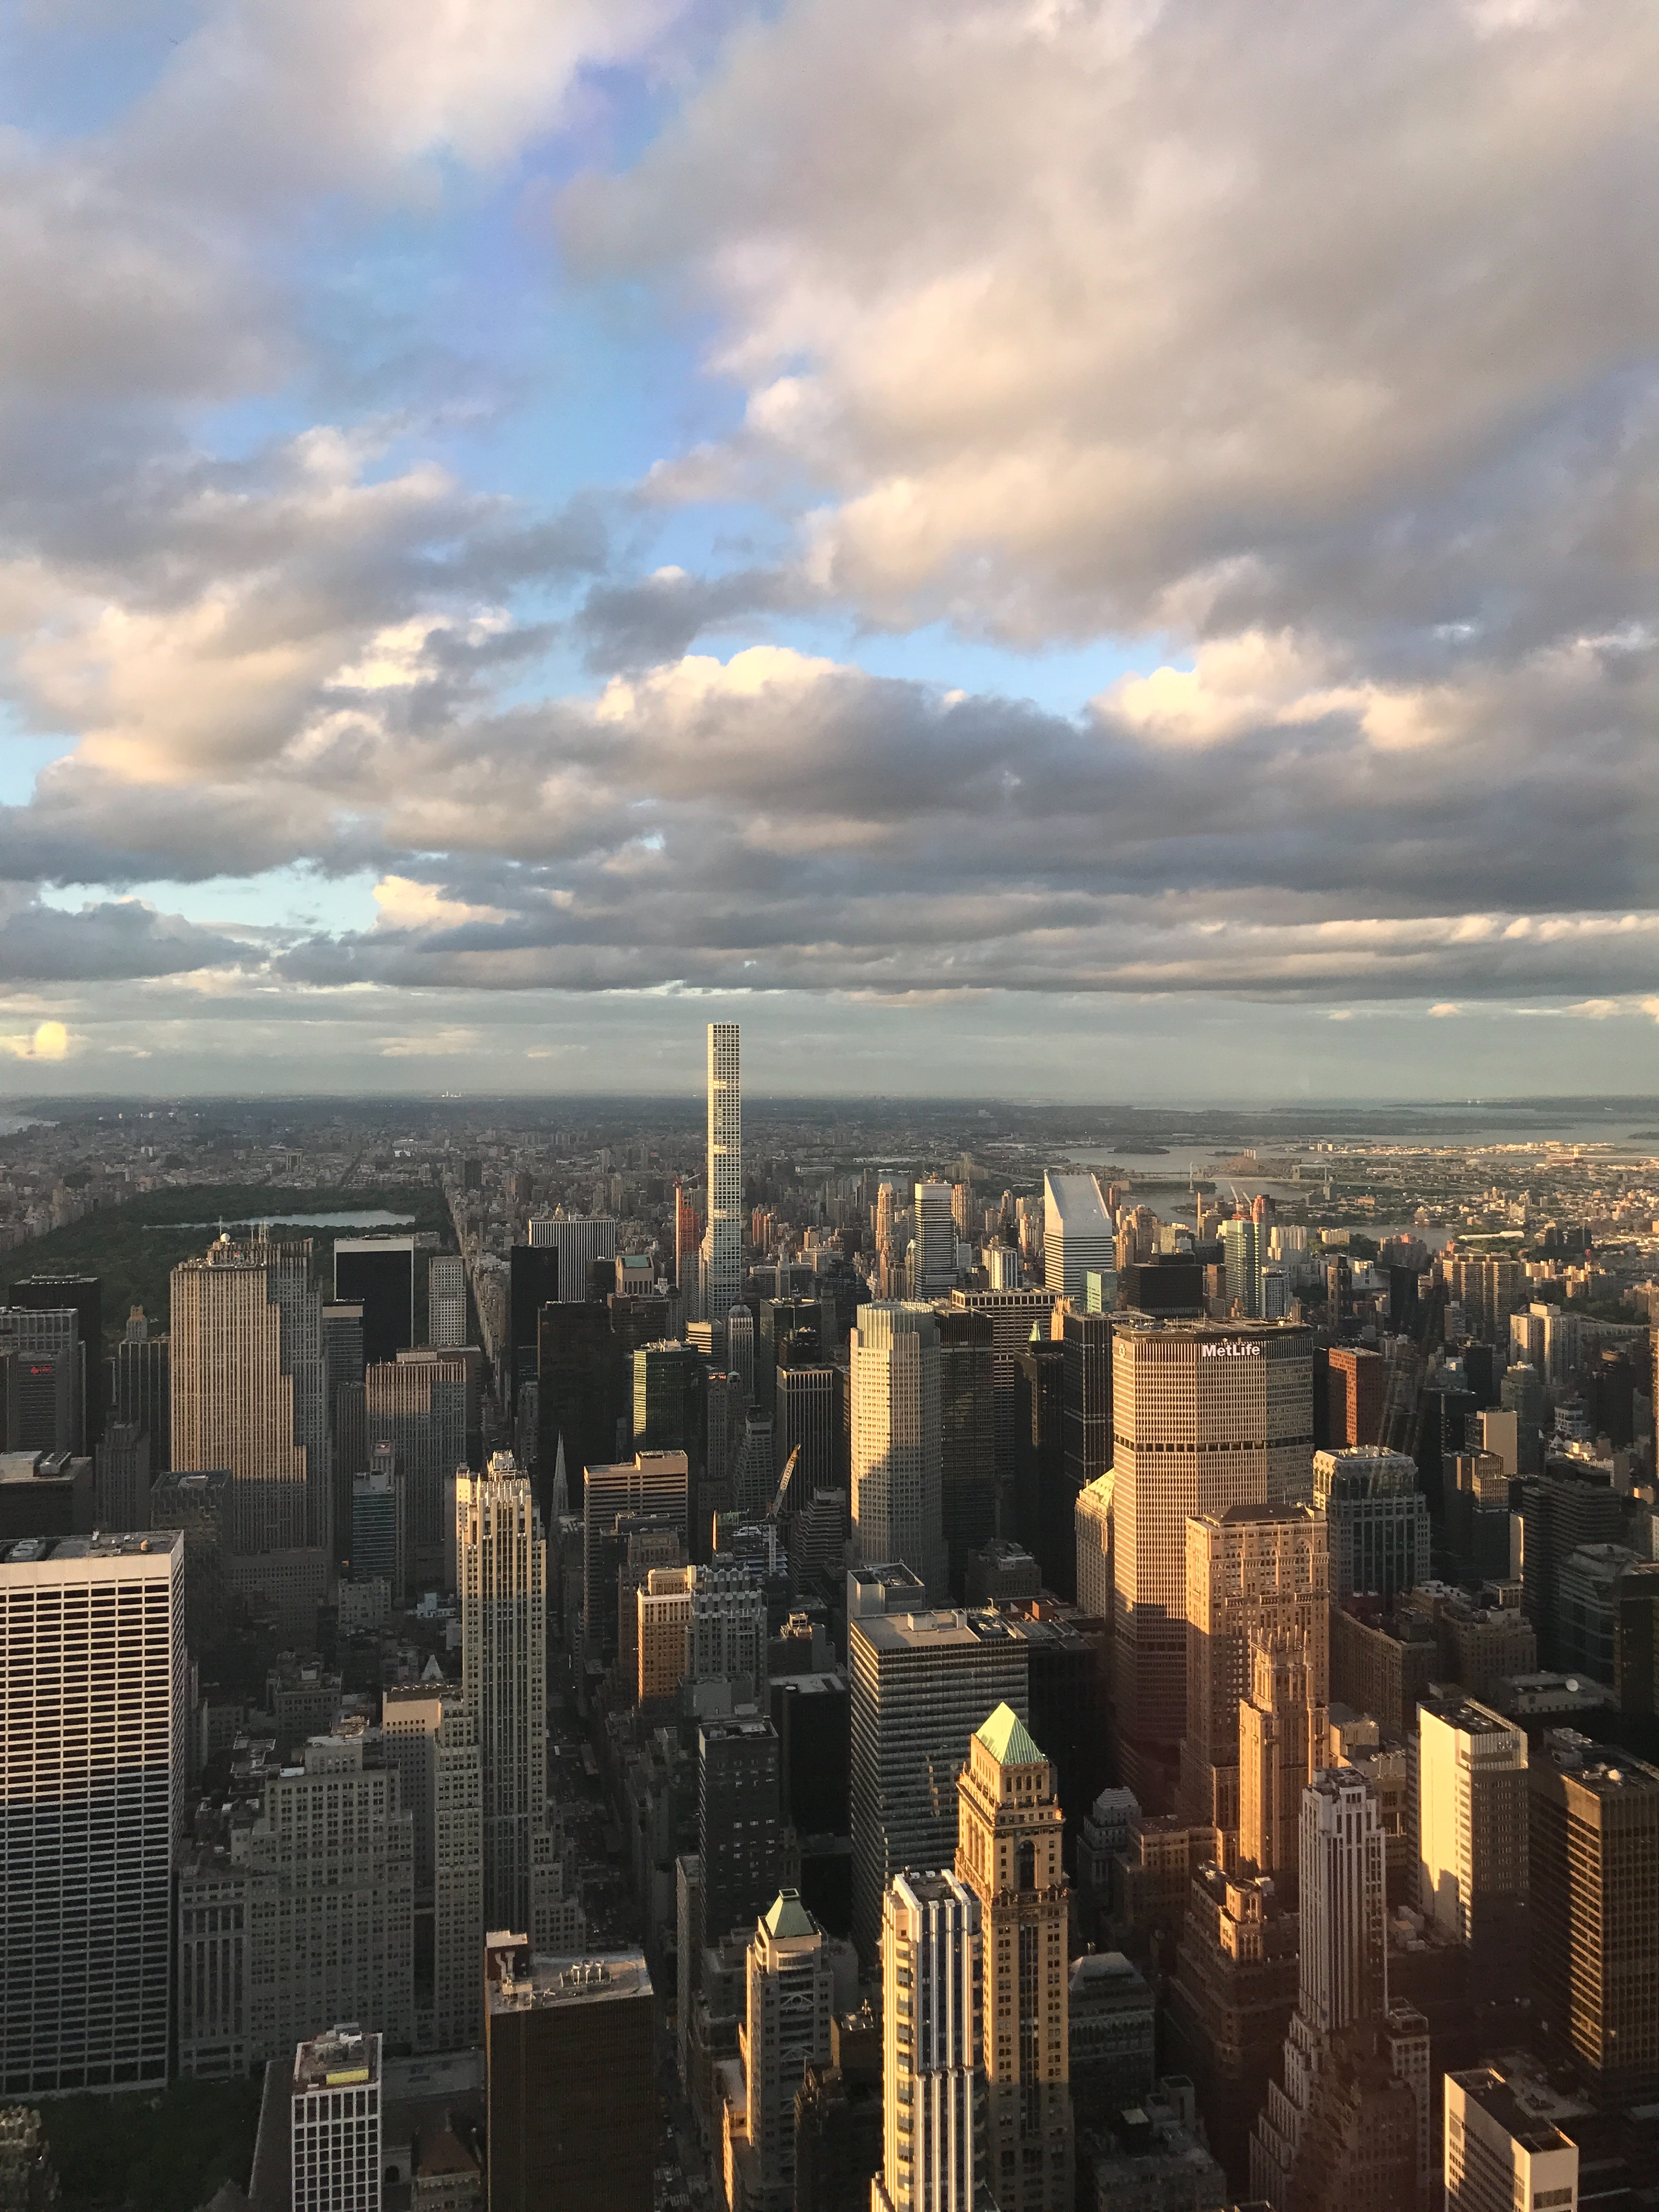
\includegraphics[height=12em]{input/new_york.jpg}}
    \subfigure[Jackson Pollock Number 30]{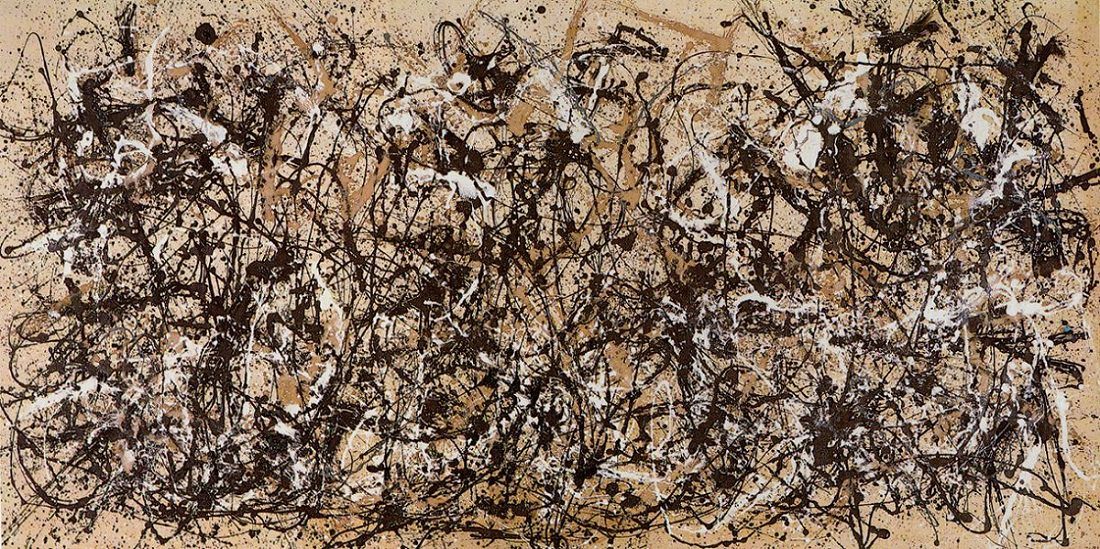
\includegraphics[height=8em]{input/jackson_pollock.jpg}}
    \subfigure[Style tranferred output]{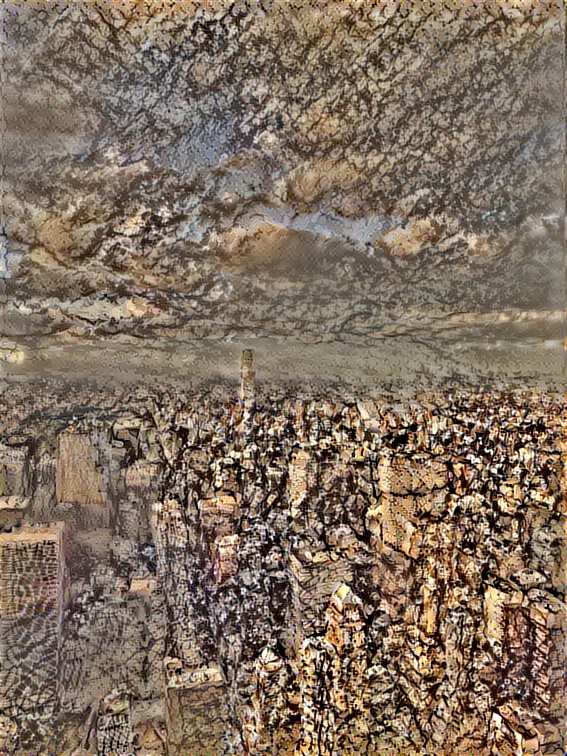
\includegraphics[height=12em]{output/jp_final.jpg}}
    \caption{Overlay Pollock on New York}
    \label{fig:results:jp}
    \end{figure}

The procedure of these two examples are the same as of the Van Gogh example.
Therefore, checkpoint output images and loss function plot are not provided here.


The reader can easily replicate the examples with the Python code appended
(see Appendix \ref{app:readme} and Appendix \ref{app:code}).
